\section{Fundamentos teóricos}
\subsection{El problema difícil de la conciencia}
Chalmers (1995) formuló el problema difícil así: ninguna combinación de magnitudes físicas, por compleja que sea, implica lógicamente la existencia de experiencia subjetiva. Todas las descripciones físicas --- neuronales, computacionales, funcionales --- describen qué hace el cerebro. No describen cómo es ser un cerebro. No describen por qué existe la experiencia. Lo que propongo: la conciencia no la genera el cerebro. El cerebro es un receptor. La experiencia es la transducción del campo akáshico.

\subsection{El monismo russelliano}
Russell (1927) observó algo profundo: la física describe las propiedades estructurales de la materia --- masa, carga, espín, posición --- pero guarda silencio total sobre la naturaleza intrínseca de aquello que porta esas propiedades. Sea S un sistema físico cualquiera: R(S) designa sus propiedades relacionales/estructurales e I(S) sus propiedades intrínsecas. La tesis russelliana afirma que I(S) es protoexperiencial para todo S.

\subsection{Integrated Information Theory}
Tononi (2004, 2008) ofrece un marco matemático para cuantificar la conciencia:
\begin{equation}
\Phi = \min_{\{P \in P\}} D_{KL}(p(X_{t+1})|X_{t}) \parallel \prod_{i} p(x_{i} \land (t+1)|x_{i} \land t))
\end{equation}
Explicación sencilla: $\Phi$ mide hasta qué punto está integrada la información en un sistema. Cuanto mayor es $\Phi$, más rica es la experiencia del sistema.

\subsection{Orchestrated Objective Reduction}
Penrose (1996) propone que las superposiciones cuánticas sufren un colapso gravitatorio espontáneo cuando la energía de superposición $E_G$ alcanza un umbral:
\begin{equation}
\tau \approx \frac{\hbar}{E_G}
\end{equation}
Lo que me interesó: la frecuencia de colapso para los microtúbulos corticales es $\tau \approx 25$ ms, lo que corresponde a $\sim 40$ Hz --- exactamente la frecuencia de las oscilaciones gamma, el marcador empírico más robusto de los estados conscientes. Apoyo experimental: Babcock et al. (2024) mostraron superradiancia ultravioleta en microtúbulos a temperatura ambiente; Kalra et al. (2023) mostraron que los gases anestésicos atenúan específicamente los efectos ópticos cuánticos en los microtúbulos.

\subsection{Kaluza--Klein y teoría F}
Theodor Kaluza propuso en 1919 la unificación de la gravitación con el electromagnetismo mediante una quinta dimensión. Einstein se entusiasmó y trabajó en esta teoría entre 1938 y 1943. La formulación original:
\begin{equation}
dS^2 = g_{\mu\nu} dx^\mu dx^\nu + \varphi^2(dx^5 + A_{\mu} dx^\mu)^2
\end{equation}

\subsection{El campo Akasha}
El concepto de Akasha (sánscrito: \emph{ākāśa}) es un elemento fundamental de la filosofía india. Akasha es el elemento más sutil, inmaterial. Es el primero que se manifestó en el universo. De él se habrían desarrollado todos los demás elementos. En la teosofía, Akasha se reinterpreta como un campo informacional universal (Laszlo, 2014). Los «registros akáshicos» registran todos los acontecimientos del universo. La hipótesis ART-12D: Akasha es el campo cuántico de la materia oscura. \textit{Nota: Akasha se usa aquí solo como metáfora de un campo físico, no como entidad religiosa.}

\subsection{Materia gris vs materia oscura}
La materia gris es el tejido del sistema nervioso central compuesto principalmente por cuerpos celulares neuronales, dendritas, terminales axonales no mielinizadas y células gliales. Es la sede del procesamiento de la información. La materia blanca está compuesta por axones mielinizados y es responsable de la transmisión.

\subsection{Una definición operativa de la conciencia}
Propongo una definición operativa que separa el contenido de la conciencia de la capacidad de integrarlo:
\begin{equation}
C_{\text{total}} = I_{\text{content}} \times C_{\text{awareness}}
\end{equation}
donde $I_{\text{content}}$ es la información estructurada (el contenido de la experiencia) y $C_{\text{awareness}}$ es la consciencia (la capacidad de saber que uno sabe). Piense en una cámara. Captura imágenes (información), pero no sabe que las captura. Una persona con una cámara captura imágenes Y sabe que las captura. Del mismo modo, la conciencia es información + consciencia.

\subsection{La convergencia con Dulcan}
Dumitru Constantin Dulcan (n. 1938), neurólogo y psiquiatra, publicó en 1981 «La inteligencia de la materia», distinguida en 1992 con el premio de filosofía «Vasile Conta» de la Academia Rumana. Las ideas que me influyeron: la conciencia no la genera el cerebro, sino que lo usa como instrumento; el subconsciente contiene la inteligencia infinita del Universo; el pensamiento es la fuerza más poderosa del universo, con una frecuencia y un campo energético propios; existe un campo de energía y luz que coordina la materia. La convergencia con ART-12D: Dulcan aporta la intuición conceptual, ART-12D aporta la formalización matemática y las predicciones testables.

\subsection{La estructura tripartita de la entidad humana}
Propongo un modelo tripartito de la entidad humana, análogo a los estados de agregación del agua:
\begin{table}[H]
\centering
\begin{tabular}{@{}llll@{}}
\toprule
\textbf{Estado} & \textbf{Entidad humana} & \textbf{Sustrato} & \textbf{Correspondencia ART-12D} \\ \midrule
Sólido & Cuerpo físico & Materia & M (materia ordinaria) \\
Líquido & Alma & Energía & E (el campo de la conciencia) \\
Gaseoso & Espíritu & Información & Sp (el campo akáshico) \\ \bottomrule
\end{tabular}
\end{table}
Formalización: $H = M + E + Sp$. Consecuencias: la muerte no destruye la entidad, solo cambia el estado dominante; la conciencia puede acceder a cualquiera de los tres estados; la enfermedad aparece cuando uno de los estados se desequilibra.

\subsection{Las formas del pensamiento como estructuras informacionales}
Los pensamientos no son solo actividad neuronal, sino estructuras informacionales que pueden tomar múltiples formas. Imaginada (visualización interna, el campo de la conciencia), pronunciada (la palabra hablada, el campo akáshico + una onda sonora), escrita (texto escrito, materia + información), dibujada (representación visual, materia + forma). Formalización general: $F_{\text{thought}} = \sum_{\text{forms}} \alpha_i F_i$.

\subsection{La empatía como resonancia de frecuencia}
La empatía puede formalizarse como un caso particular de telepatía, en el que el acoplamiento es emocional y no informacional. Formalización:
\begin{equation}
\text{Empathy}(A,B) = \frac{1}{1 + \frac{(\omega_A - \omega_B)^2}{\Gamma^2}}
\end{equation}
Interpretación: cuando las frecuencias coinciden ($\omega_A = \omega_B$), la empatía es máxima; cuando difieren, la empatía disminuye; la empatía no depende de la distancia (el campo es omnipresente). Predicción testable: las parejas con alta empatía deberían mostrar correlaciones EEG más fuertes que las parejas con baja empatía.

\subsection{La palabra como excitación del campo akáshico}
Propongo que la materia oscura tiene una manifestación acústica --- un espectro de oscilaciones que pueden ser excitadas por ondas sonoras. La motivación cosmológica: las oscilaciones acústicas primordiales (BAO) son fluctuaciones de la densidad de materia que se propagaron como ondas sonoras en el universo temprano. En ART-12D, esas oscilaciones son oscilaciones del campo akáshico. Formalización:
\begin{equation}
A(x,t) = \sum_n A_n \cos(\omega_n t + \varphi_n)
\end{equation}
El espectro acústico:
\begin{equation}
\omega_n = \frac{1}{R} \sqrt{n^2 + \mu_A^2 R^2}
\end{equation}
El acoplamiento palabra--campo:
\begin{equation}
L_{\text{int}} = g_{\text{sound}} A \cdot \Phi_{\text{sound}}
\end{equation}
Efectos diferenciados: Amor (200-400 Hz, activa las zonas emocionales positivas), Miedo (500-800 Hz, activa la amígdala), Sanación (300-500 Hz, activa la expectativa positiva), Muerte (150-300 Hz, activa las zonas de ansiedad).

\textbf{El problema de escala.} El espectro acústico $\omega_n$ viene fijado por el mismo radio de compactificación que da su masa a la materia oscura. Para $1/R = 10^{-5}$ eV, los modos están en la gama de los GHz, no en centenares de Hz. Una resonancia a 150--800 Hz exigiría $1/R \approx 1,24\times10^{-12}$ eV, unos siete órdenes de magnitud por debajo de la escala de masa. Mientras no se introduzca una segunda escala de compactificación, la predicción no tiene contenido numérico: el acoplamiento $g_{\text{sound}}$ no está fijado de forma independiente.

\begin{figure}[H]
\centering
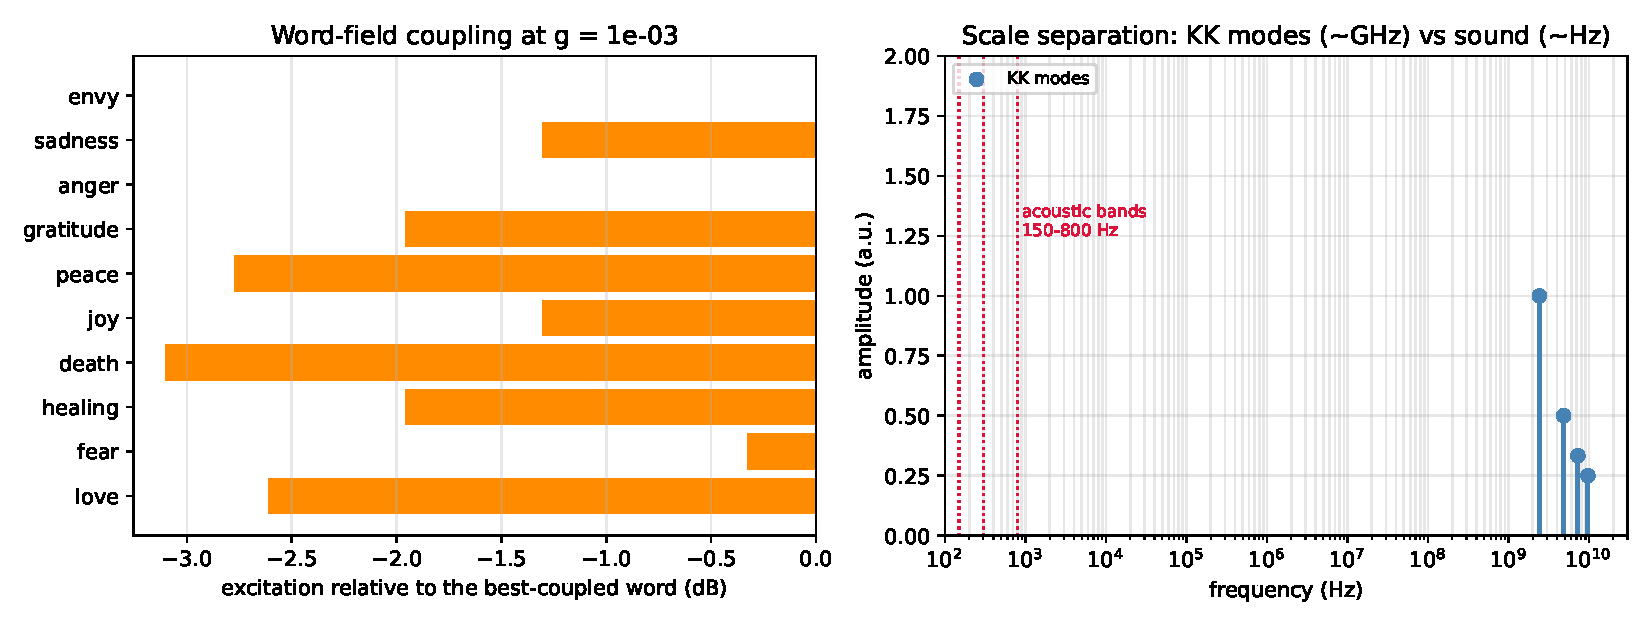
\includegraphics[width=0.9\textwidth]{figures/fig06_word_excitation.pdf}
\caption{Izquierda: el acoplamiento relativo palabra--campo para las diez bandas usadas en el artículo. Derecha: la separación de escala entre los modos KK (~GHz) y las bandas acústicas (~Hz).}
\label{fig:cuvant}
\end{figure}

\subsection{El tiempo como vibración}
La definición del segundo: «Un segundo es la duración de 9.192.631.770 periodos de la radiación del átomo de cesio-133». Qué ocurre si la frecuencia cambia: si la frecuencia aumenta, el tiempo se comprime; si disminuye, el tiempo se dilata. La resonancia de Schumann: históricamente $\sim 7,83$ Hz, recientemente $\sim 12$ Hz. El corazón como reloj biológico: miedo ($\sim 120$ bpm) --- el tiempo vuela; meditación ($\sim 50$ bpm) --- el tiempo se dilata; sueño profundo ($\sim 40$ bpm) --- el tiempo desaparece. Referencias relativas, no absolutas: el cesio (9.192.631.770 Hz), Schumann (7,83--12 Hz), el corazón (1,2 Hz). Todas son relativas. Ninguna es «la verdadera».
\begin{equation}
\text{Reality} = \frac{\text{Change}}{\text{Reference}}
\end{equation}

\subsection{Realidades múltiples y el multiverso}
El campo akáshico total: $A_{\text{total}} = \sum_{k=1}^{N_{\text{vacua}}} A_k$. El estado del multiverso: $|\Psi_{\text{multiverse}}\rangle = \otimes_{k=1}^{N_{\text{vacua}}} |A_k\rangle$. La intersección de realidades: las realidades no son solo paralelas --- pueden intersectarse.

\subsection{La biblioteca universal (Akasha)}
El contenido del campo: el campo akáshico contiene toda la información --- todo lo que fue, todo lo que es, todo lo que será.
\begin{equation}
A_{\text{total}} = \sum_{\text{(all events)}} A_i
\end{equation}
El acceso a la información:
\begin{equation}
I_{\text{access}}(t) = \int_0^\infty S_A(\omega) S_G(\omega, t) d\omega
\end{equation}
La indexación: la información se indexa por relevancia, no por tiempo.
\begin{equation}
\text{Information received} = \text{Akashic field} \times \text{Relevance}(t)
\end{equation}

\subsection{La jerarquía de la recepción}
\begin{table}[H]
\centering
\begin{tabular}{@{}clcc@{}}
\toprule
\textbf{Nivel} & \textbf{Sistema} & \textbf{$\Phi$} & \textbf{Acceso} \\ \midrule
0 & Termostato & 0 & Ninguno \\
1 & C. elegans & Mínimo & Quimiotaxis \\
2 & Insecto & Bajo & Sensación \\
3 & Ratón & Moderado & Emoción \\
4 & Perro & Alto & Empatía \\
5 & Córvido & Alto & Planificación \\
6 & Octópodo & Distribuido & Resolución \\
7 & Humano & Muy alto & Autorreferencia \\
8 & Humano entrenado & Extendido & Metacognición \\ \bottomrule
\end{tabular}
\end{table}
El límite de la recepción: $\lim_{\Phi \rightarrow \infty} E(\Phi) = I_{\text{total}}$.

\subsection{La palabra como origen: la convergencia de las religiones}
Todas las grandes tradiciones religiosas describen la Palabra como origen del universo. El cristianismo tiene el Logos --- la Palabra (el modo fundamental del campo). El hinduismo tiene Om (la vibración primordial). El islam tiene Kun («¡Sé!»).

\subsection{La manifestación acústica del campo akáshico}
$A(x,t) = \sum_n A_n \cos(\omega_n t + \varphi_n)$. El espectro acústico: $\omega_n = \frac{1}{R} \sqrt{n^2 + \mu_A^2 R^2}$.

\subsection{Dios en ART-12D}
Hay cuatro hipótesis. Dios es el campo akáshico mismo. Dios es la fuente del campo. Dios es la conciencia universal. Dios es una proyección humana. No sé cuál es la correcta. Pero la pregunta es legítima.

\subsection{Materia oscura y energía oscura: dos caras del mismo campo}
La hipótesis ART-12D: la materia oscura y la energía oscura son dos aspectos del mismo campo akáshico. Formalización:
\begin{equation}
L_A = \frac{1}{2} g^{MN} \partial_M A^* \partial_N A + \frac{1}{2} \mu_A^2 |A|^2 - \frac{\lambda_A}{4} |A|^4
\end{equation}
La ecuación de estado: $w = p_A / \rho_A$. Para un campo oscilante, la media temporal se calcula exactamente sobre la órbita y depende de la relación $\delta = A_{\text{osc}}/A_{\min}$ entre la amplitud de oscilación y el valor del potencial en el mínimo. Hay tres regímenes distintos:
\begin{center}
\begin{tabular}{@{}lll@{}}
\toprule
\textbf{Régimen} & \textbf{Condición} & $w$ \\ \midrule
Oscilación pequeña en torno al mínimo & $\delta \ll 1$ & $0$ (materia) \\
Oscilación dominada por el término cuártico & $\delta \gg 1$ & $1/3$ (radiación) \\
Campo congelado en el mínimo & $\delta = 0$ & $-1$ (constante cosmológica) \\ \bottomrule
\end{tabular}
\end{center}
La versión 30 afirmaba que el régimen de gran amplitud da $w \simeq 1$. El valor correcto es $1/3$: el teorema del virial da $\langle K \rangle = 2\langle V \rangle$ para un potencial dominado por el término cuártico. El valor $w = 1$ corresponde a una dominancia cinética (kination), que las oscilaciones cuárticas no alcanzan, mientras que $w = -1$ corresponde al campo congelado, no a una amplitud pequeña.
